\chapter{Filesystem Metaphore and the Pipe Abstraction}
From our experience with building applications, there are a clear set of requirements that are necessary.  Most applications
construct the notion of context using the naming convention ascribed to a sensor stream.  The name conflates the notion of system,
space, and type information.  At the very least, these three should be supported, however, often other categorical needs must be
met to perform various kinds of aggregate statistical, analytics, and control.  In addition, we need to support the management of
processing jobs that process stream data and provide integrated management facilities for them.

Building applications are essentially monitoring and control applications built on the streams generated by sensors embedded through
the building or distillates of them.  As the number of applications and streams increased, it becomes desireable to manage them 
in a centralized fashion.  Moreover, the centralized apporach allows all applications to make use of a uniform naming convention and
can allow applications to be interoperable.  Systems that wish to support such applications require the following properties:

\begin{enumerate}
\item Logically accessible physical resources.
\item Representation of data producing and data consuming elements.
\item Representation of inter-relationships between elements.
\item Provide uniform naming and access.
\end{enumerate}

This chapter describes the use of the filesystem and pipe abstraction for represents streams in space.  The filesystem naming convention
provide a a unified namespace to application, for accessing physical resources and streams.  Moreoever, we support multi-naming through
symbolic links -- an important requirement for building applications.  We also discuss the incorporation of a pipe-like mechanism for 
processing streams and their output.


\section{Related Work}
HomeOs~\ref{homeos}


\section{File abstraction and Supporting Multiple Names}
Similar requirements to those aforementioned have been addressed in the design and implementation of filesystems.  Filesystems provide
logical access to physical resources through files, with different files and associated semantics, exposed to applications through a shell
or programmtically.  Filesystems representat collections of bits, encapsulated by a file, and grouped with folders.  Symbolic links support
the notion of multi-naming.  A single file or folder could have multiple names that lead to the same underlying object.  Filesystems even
support the notion of streaming data through character and block device files.  Moreover, pipe files allow programs to communite with each
other through a piece of shared memory, where the source application writes to the pipe and the sink application consumes from the pipe.

We assert that these constructs should be directly adopted for supporting applications in the buildings.  Our approach adopts the unix
file philosophy where everthing is represented as a file.  Each object created in StreamFS is assigned two names, by default, one which 
uniquely identifies the object and \emph{not} human-readable and the second which is changeable and human-readable.  Consider
the example shown in Figure~\cite{fig:everythingfile}.


\begin{figure}[t!] %htbp
\centering
\includegraphics[width=0.65\columnwidth]{figs/everythingfile}
\caption{Everything is a file.  Temperature sensor represented as a file in a folder that contains folders for each room.
Note, the file that represents a temperature sensor producing a stream is given a unique identifer.  The user may also
decorate the file with extra metadata for searching purposes.}
\label{fig:everythingfile}
\end{figure}

In this example, the user is creating a temperature stream file in every room of the building.  The name of the file, given by the user,
is \emph{temp}.  Upon creation, the file is uniquely identified by the system using a unique identifier, as shown.  Like in a unix filesystem, the
file is created within a folder.  Ideally, the name of the folder would encode the placement of the sensor.  In the figure, the 
user is create a temperature stream file in room 410 and room 420.  Note the full filepath for the stream file is /room/410/temp.
During creation, the user may also decorate the file with extra metadata, also shown in the figure.  In this example, they have annotated
the file with information about the owner and when the sensor was installed.   This metadata is used for quickly locating the file
or grouping files that contain similar tags, quickly.

\subsection{File types and operations}
As we map the filesystem abstraction into this problem space, we need to consider the various kinds of files our system will contain,
their semantics, and how our system will expose and manage them.  There are essentially 4 types of files and 6 sub-types.  We summarize
these in Table~\ref{tab:filetypes}


% \begin{enumerate}
% \item default/folder
% \item stream
% \item contoller
% \item special file
% 	\begin {enumerate}
% 		\item internal process definition (ipd)
% 		\item internal process instance (ipi)
% 		\item external process information (epinfo)
% 		\item external process instance (epi)
% 		\item subscription instance (sub)
% 		\item symbolic link (symlink)
% 	\end{enumerate}
% \end{enumerate}


\begin{table}[h]
\begin{center}
\begin{tabular}{| r | l | c |}
	\hline
	\textbf{type} & \textbf{description} & \textbf{valid operations} \\ \hline
	default/folder & Container file.  Used to group other  & read, write, delete  \\
				   & kinds of files within it.  &  \\

	stream & Represents a data stream. & read, write, delete, subscribe, query \\

	controller & Represents a controller. & read, write, subscribe \\

	special & There are several kinds of special files for  & read, delete \\
		    & management of jobs and pipes. &  \\
	\hline
\end{tabular}
\caption{Summary of the 4 main file types and their valid operations in StreamFS.}
\label{tab:filetypes}
\end{center}
\end{table}



\begin{table}[h]
\begin{center}
\begin{tabular}{| r | l | c |}
	\hline
	\textbf{type} & \textbf{description} & \textbf{valid operations} \\ \hline
	internal process defintion (ipd) & Javascript process definition.  & read, write, delete  \\

	internal process instance (ipi) & Management file used for managing & read, delete \\
							  & active processing of this script. & \\

	external process definition (epd) & Gives information about where an & read, write, delete \\
								& external process lives. &\\

	external process instance (epi) & An active processing stream to an  & read, write, delete \\
								& external process. &\\

	subscription instance (sub) & An instance of a subscription.  Contains & read, delete \\
								& information about the subscription, &\\
								& such as source/sink and related statistics &\\
	symbolic link (symlink) & Similar to a symbolic link in Unix. & \\
	\hline
\end{tabular}
\caption{Summary of the 6 special-file sub-types and their valid operations in StreamFS.}
\label{tab:filesubtypes}
\end{center}
\end{table}


\begin{table}[h]
\begin{center}
\begin{tabular}{| r | l | l |}
	\hline
	\textbf{operation} & \textbf{file type} & \textbf{semantics} \\ \hline
	read & folder, stream, ipd, ipi, epd, epi, sub & read the metadata and tags for \\
		 &										   & the associated file. \\
	write &  folder, stream & Write to metadata of folder and stream. \\
		& 					& Write to stream file.\\
	delete & folder, stream, ipd, ipi, epd, epi, sub & Folder must be empty.  The others can be directly deleted. \\
	query &  stream & \\
	subscribe & stream & \\
	\hline
\end{tabular}
\caption{Summary of the 6 special-file sub-types and their valid operations in StreamFS.}
\label{tab:semantics}
\end{center}
\end{table}





\section{Processing Pipelines and Management}
	\subsection{Entity Relationships}
\section{Internal Processes}
\section{External Processes}
\section{API Overview}
	\subsection{RESTful API}
	\subsection{Programmatic API}
\section{Example Application: Deployment Viewer}
\section{Example Application: Mounted Filesystem and Matlab Integration}
\section{Summary}


\chapter{Process Management and Scheduling}
Data is coming in at different, independent rate from sensors and is produced asynchronously from internal processing elements.
For certain processes, processing the incoming data as quickly as possible is key, however, this is challenging for several reasons:
1) a process may subscribe to multiple, independent streams with asychronized report schedules and 2) interpolated values
should be avoided to minimize prediction inaccuracies in interpolated values.  Therefore, a process actually wants all the freshest
data from all the streams they are subscribing to, while minimizing the average time that the data for each respective stream has 
been waiting in the buffer.


\section{Related Work}
\section{Designing for Horizontal Scalability}

%\section{Minimizing Data Time in Buffer}
\section{Maximizing Data Freshness}
Certain jobs only care about consuming the latest readings from their subscription streams.  They are willing to discard reading until two
conditions are met:

\begin{enumerate}
\item There is at least one data point from each stream in the subscription buffer.
\item The statelness factor is minimized within the immediate time window.
\end{enumerate}

This is of particular interest to controllers that need to make control decision based on the freshest data possible and can tolerate some variability
in the completion time of the control task.  It is also useful in analytical jobs that want to process the latest data from multiple streams while also
allowing some variability in the completion of the processing task.  Note, there's a fundamental tradeoff
between the staleness factor and variability of consumption.  It is sometimes better to wait for the next incoming data point than it is to use what
is currently in the buffer, as waiting will decrease the overall staleness factor.  Other times, it is better to consume the bufferred data immedaitely.
This causes a certain amount of variability in the delivery period to the control process.  However, for some applications, this is a reasonable tradeoff
to make.  Making use of the freshest data is desirable for minimizing errors, either in the control of a system or the calculation of some aggregate state.
Generally, the error grows with staleness, therefore the goal of this mechanism is to continuously minimize the error associated with staleness through
scheduling.


\begin{figure}[t!] %htbp
\centering
\includegraphics[width=0.75\columnwidth]{figs/min_buffer}
\caption{Multiple streams in a subscription and their associated parameters.}
\label{fig:min_buffer}
\end{figure}

Let $A_{i}$ be the arrival time of the last data point received from stream $i$ and $D_{i}$ be the arrival time for the next data point from stream $i$
and their relationship as described in equation \ref{eqn:deadline}, where $T(i)$ is the average period between the arrivals from stream $i$.

\begin{equation}
D_{i} = A_{i} + T(i)
\label{eqn:deadline}
\end{equation}


Periodically, our algorithm runs and checks if there is a data point for each stream in the subscription.  If so, the \emph{min\_buffer} algorithm runs 
and effectively decides whether to execute the job on the current buffer immediately or whether to wait until later, when the \emph{staleness factor} of
the buffer will be at a minimum.  This decision is driven by equation~\ref{eqn:later_better_condition}, whereby we find the next deadline, computed with
equation~\ref{eqn:last_deadline}, for each stream in the set and determine the staleness factor will be for the entire buffer if we wait until that deadline arrives.

\begin{equation}
t_{L,i} = A_{i} + \Bigl\lfloor \frac{D_{k}-A_{i}}{T(i)} \Bigr\rfloor T(i)
\label{eqn:last_deadline}
\end{equation}

If there is no deadline $D_{k}$ for some stream $k$ such that equation~\ref{eqn:later_better_condition} holds, then we execute now.  Otherwise we choose to wait
until $D_{k}$ for the stream whose next deadline minimizes the staleness factor of the buffer.


\begin{equation}
\sum_{i=1}^{k-1} D_{k} - t_{L,i} < \sum_{i=1}^{k} t_{now} - A_{i}
\label{eqn:later_better_condition}
\end{equation}

The algorithm is sketched our below.


\begin{algorithm}[h!]
 \SetAlgoLined
 Given a full buffer $b[n]$:\\
  \For{all elements in the $b$}{
  (1) Calculate the staleness of element $i$ and add to total stalness, $S_n$\;
  \For{all other elements in the buffer}{
  	(1) Determine the next report time $D_i$ for this element\;
  	(2) Determine the staleness of all the elements if we wait until $D_i$\;
  	(3) If it is the smallest staleness figure calculate, replace minimum cost, $S_l$.
  	}
  }
  \If{$S_l$ is less than $S_n$}{
  (1) Wait until later to consume\;
  \Else{
  (1) Consume now}
  }
 \caption{Staleness algorithm.}
 \label{alg:emd}
\end{algorithm}

\section{Experimental Results}

\begin{figure}[t!] %htbp
\centering
\includegraphics[width=0.9\columnwidth]{figs/staleness_vs_numstreams}
\caption{}
\label{fig:stalevsstreams}
\end{figure}

\begin{figure}[t!] %htbp
\centering
\includegraphics[width=1.0	\columnwidth]{figs/period_vs_streams}
\caption{}
\label{fig:report_periods}
\end{figure}


\section{Summary}




% \chapter{Metadata Evolution and Verification}
% \section{Verication through Sensor Data}

% \section{Types of Verification}
% \subsection{Geometric Verification}
% \subsection{Functional Verification}
% \subsection{Value Verification}

% \section{Structural Verification With Empirical Mode Decomposition}

% \subsection{Introduction}
Buildings consume an enormous amount of energy in countries around the world.  In 
Japan, 28\% of the energy produced is consumed in buildings~\cite{japanbuildings} while in the United 
States it is as high as 40\%~\cite{epabuildings}.  Moreover, studies show that between 30-80\% of it
is wasted~\cite{waste_science, next10_waste}.  Large commercial buildings are typically instrumented
with a large number of sensors measuring various aspects of building operation.  Although this data is
typically used to assure operational stability, they may also be used to measure, observe, and identify
instances of wasted use.

Identifying instances of wasted energy use is non-trivial.  System efficiency is defined as the ratio of the 
useful work done to the energy it consumes.  In the case of buildings, we broadly define useful work as 
the energy used to support occupant activities.  From the perspective of the building that means maintaining
a comfortable temperature setting, providing power for plug-load devices, and providing adequate lighting
conditions; particularly in spaces that are occupied.  However, identifying efficient use of resources,
\emph{especially} when a space is occupied, is difficult.  Typically it involves deep knowledge of the usage scenario and
a meaningful understanding of what it takes to support the activity.  Furthermore, situations and activities differ
greatly.  The outside weather changes, varying schedules affect occupancy, rooms have lectures, class,
or other office activities.  Simply put, the process is time consuming, requires specialized knowledge,
and does not scale.

Devices are typically used together in some fashion.  For example, in an office
setting a person enters their office, turns on their PC and lights, etc.
When the person leaves the office, they revert back to the state their devices were in before arrival.
If one of the items is not reverted to its pre-arrival state, waste occurs. 
%Waste occurs when something is left on.
The same is true about equipment usage.  When the outside temperature is low the heater turns on.
% and
%the negation is also true.  If the temperature is high and the heater is on, waste occurs.  
\emph{Waste occurs when abnormal in-concert usage patterns arise}.  
%For example, 
% Moreover, if the heating and cooling system are on 
% simultaneously~\cite{simheatcool}, that is a problem that is \emph{particularly} wasteful and hard to 
% detect by occupants.  
Fundamentally, understanding ``normal'' spatio-temporal usage patterns between devices could help
identify problems when devices are not being used correctly.
We conjecture that inefficient energy use can be identified through anomalies in the correlation
patterns between devices.  We examine device correlation patterns in this paper and look specifically
at processing raw sensor traces, such that the correlations we find are meaningful.

In this paper, we present early results for correlating usage patterns across a large number of sensors
in a single deployment.  We analyze data from a 12-story office building at the University of Tokyo.  
The deployment consists of almost 700 sensors monitoring a broad range of devices inside and outside 
the building.  Our initial observations and results include the following:

\begin{enumerate}
\item Raw-trace correlation analysis is too strongly influenced by the common low-frequency trends in the data
	to identify meaningful relationships.
\item Using a technique called empirical model decomposition (EMD)~\cite{huang:emd1998} removes this 
		 trend and helps identify truly correlated sensor traces.
\item We can construct clusters of correlated sensors that are spatio-temporally correlated, \emph{without
		a priori knowledge of their placement}.
\end{enumerate}

In the rest of the paper we explain EMD and how we use it, we show various examples of our technique on real-world
traces, and we discuss the implications and future work.

% Green IT

% Understand the energy consumption of a building and identify savings opportunities.

% Identification of energy consuming devices that are correlated.
% Uncover usage patterns of correlated device that are energy efficient.
% Detect deviation from the energy efficient pattern and report to the user.

% During the design of our application the first difficulty was to identify the set of devices that have related energy consumption.

% This article focuses on this problem.

% Results:
% \begin{enumerate}
% \item Correlation is noisy and can't find inter-relationships between sensors
% 		with subtle differences.
% \item Underlying behavior should extract most-common denominator in comparing traces
% 		to observe truly correlated behavior.
% \item Empirical mode decomposition (EMD) can be used to compare underlying behavior after the
% 		removal of the dominant frequencies in the signal.
% \end{enumerate}

% \subsection{ideas}

% Future work:
% \begin{enumerate}
% \item We can create a time-varying dependency graph to compare ``normal'' versus ``abnormal'' behavioral
% 		patterns in underlying use.
% \item We can codify ``normal'' or ``efficient'' graphs and compare with real graph constructs over time.
% \end{enumerate}

% Possible algorithms:
% \begin{enumerate}
% \item find correlated and uncorrelated sensors
% \item construct correlation network where the nodes are the sensors and an edge implies correlation above
% 		threshold. (We can also construct the complement of that.)
% \end{enumerate}


% \section{Related work}

\begin{itemize}
\item dashboard
\item andrew's lightin control work
\item Kamin's hvac control work
\item BEMs
\item sMAP stuff
\item Buildsys 2010 work~\cite{hbci}
\end{itemize}
% \subsection{Dataset}
The data we used was obtained from a deployment of sensors in a 12-story office building
on the campus of the University of Tokyo~\cite{gutp, ogawa:lncs2011}.  The deployment consists of 
almost 700 sensors monitoring device power consumption, ranging from plug-load devices to components of the
heating, ventilation, and air conditioning system (HVAC) and lighting.  Sensors also reported temperature, 
pressure, device-state, and other information.  Each sensor reports data on the
order of minutes.  Over 500 GBs of data was collected over a 2-year span.

\begin{figure*}[tb]
\hspace{-2cm}
\includegraphics[width=1.2\textwidth]{figs/emd_25_26-eps-converted-to}
\vspace{-1cm}
\caption{Decomposition of the EHP and light trace using bivariate EMD. IMFs correlation coefficients highlight the intrinsic relationship of the two traces.}
\label{fig:emd}
\end{figure*}

% The intent of the Green University of Tokyo Project (GUTP) \cite{gutp} is to reduce the university environmental impacts associated to its electric energy consumption.
% The first step of this project was to deploy sensors at the Building No.2 of the Faculty of Engineering 
% Electric power consumption of a 12 floors building containing researchers office and classroom.
% 1215 sensors monitoring different devices...

%received attention in the past \cite{ogawa:lncs2011}.

For this investigation, we focus on a three-week span in the summer of 2011 (from July 4th to July 24th).
The dataset captures regular work days, weekends, and one holiday (July 18th).  This timeframe captures
the typical usage of the equipment, triggered by occupant activity.  For the initial
analysis, we focus on three sensors; two water pumps and a light feed.  The first pump is an 
``electric heat pump'' and is labled as EHP, the second  is a ``gas heat pump''
and labeled as GHP.  The room lighting system serves the same room as the EHP.  The GHP
serves a different room on the same floor.  The expanded portion of our analysis pivots around the EHP
and does a pairwise comparison between it and all other sensors in the building.
Computationally, this approach does not scale to a large number of sensors.  For future work, we will
examine various heuristics to narrow the search space before running pairwise comparisons.

% includes one day holiday (July 18th)
% 3 different sensors:
% \begin{itemize}
%  \item Two are measuring the electric power consumption of two devices from the same room; an electric heat 
%  		pump (EHP) and the room lighting system.
%  \item One is measuring the electric power consumption of a gas heat pump (GHP) that is pumping water to cool 
%  		a different room in the same building.
% \end{itemize}

% Later we expand our analysis to include all the sensors in the building.


\subsection{Problem statement and Initial approach}\label{problem}
% In our analysis, we are focused on finding devices that are correlated in their use over time.  Therefore, the
% main objective is to examine how device traces relate to one another.  The wish to identify
% correlated device-trace patterns at large spatio-temporal scales.

In buildings, metadata is poorly and unsystematically managed within a single system domain.  Moreover, 
with the ever growing number of additional sub-meters, it is important to quickly integrate
sensor data from multiple systems to understand the full state of the building.  It is also important to 
understand how sensors are used in concert.  Anomalies in usage may indicate underlying problems with 
the equipment or inefficient/incorrect usage.  

Figure \ref{fig:raw} shows the raw traces for the three devices discussed in 
the previous section (EHP, GHP, light). All three exhibit a diurnal usage pattern.  On weekends, each
draw less power.   For our initial analysis, we calculated the pairwise 
correlation coefficient for all sensors in the set.  The correlation coefficient for 
 the EHP and light is $0.7715$ and the correlation coefficient for the EHP and GHP is $0.6370$.
Running correlation across them yields high correlation coefficients, mostly
due to their underlying daily usage pattern.


% \begin{figure}[t!]
% \centering
%  \subfigure[EHP trace]{\label{fig:raw_ehp}\includegraphics[width=.4\textwidth]{img/25.png}}
%  \subfigure[Light trace]{\label{fig:raw_light}\includegraphics[width=.4\textwidth]{img/26.png}}
%  \subfigure[GHP trace]{\label{fig:raw_ghp}\includegraphics[width=.4\textwidth]{img/41.png}}
%  \caption{Traces from three different sensors captured in 2011 from July 4th to July 24th. Data is normalized and aggregated into 30 minutes time bins.}
%  \label{fig:raw}
% \end{figure}


Our initial results were not surprising.  The diurnal pattern dominates the comparison between the sensors.
Weather is the main driver for this behavior and it affects the readings in almost all of the
sensors in our dataset.  Cross-correlation on raw sensor data is insufficient for filtering intrinsically related
behavior.  Upon closer examination of the data we assess the following:

\begin{itemize}
\item The main underlying diurnal trend occurs in almost all the traces.
\item Occupancy and room activities occur at random times during the day and change 
		at a higher frequency than weather patterns.
\item Sensors that serve the same location observe the same activities.  Therefore, their underlying
		measurements should be correlated.
\end{itemize}

In order to uncover these relationships we must remove low-frequency trends in the traces and
compare the readings at high frequencies.

% \begin{table}
% \begin{center}
% \begin{tabular}{|l|l|l|l|l|l|}
% \hline
% × & Raw trace & 1st IMF & 2nd IMF & 3rd IMF & Residual\\ \hline
% EHP, Light & 0.7715 & 0.43909 & 0.49344 & 0.63469 & 0.82132 \\ \hline
% EHP, GHP & 0.6370 & 0.0060274 & 0.063546 & 0.16764 & 0.79378 \\ \hline
% \end{tabular}
% \caption{Correlation coefficients of the analyzed trace and their IMFs uncovered by EMD}
% \label{tab:corr}
% \end{center}
% \end{table}
% \subsection{Simple Scenario}

\begin{figure*}[tb]
\hspace{-2cm}
\includegraphics[width=1.2\textwidth]{figs/emd_25_41-eps-converted-to}
\vspace{-1cm}
\caption{Decomposition of the EHP and GHP trace using bivariate EMD. IMFs correlation coefficients highlight the intrinsic independence of the two traces.}
\label{fig:emd2}
\end{figure*}

% The small difference between the two computed correlation coefficients is misleading as one could conclude that the three signals are correlated and the corresponding devices are activated by a single action.

% The high correlation coefficients obtained for these three signals result .... weekly pattern....
% small difference = local fluctuation...

% this high score comes from the fact that the two devices are monitoring offices that are weekly used.

% Indeed the weekly pattern of the data trump the correlation coefficients....

% How to inspect only the local fluctuations...?
% we'd like to have an elegant solution (i.e. not specifying the interesting time scale)


% 


\section{Methodology}\label{method}
%Remove the weekly trend of the data to analyze the detailed changes that convey the device behavior at small time scales.

% Our initial approach examined correlation analysis on raw sensor traces.  However, we quickly
% found that correlation is overly sensitive to fluctuations in the data.
Fundamentally, the readings are driven by the same underlying phenomena: 
weather and occupancy.  Weather influences \emph{all} the data similarly.  Occupancy, however, changes
throughout the building and should be used as a differentiating component in the signal
comparisons.  Sensors that share spatio-temporal elements should be correlated after the removal
of the underlying trend driven by the weather.  In order to find unique relationships we need to remove 
this common trend.

\subsection{Empirical Mode Decomposition}
Empirical Mode Decomposition (EMD) \cite{huang:emd1998} is a new technique used for de-trending data.
Specifically, EMD detrends non-stationary, non-linear timeseries data.  
% A trend is defined as 
% an intrinsically determined monotonic function within a certain temporal span or a function in which there 
% can be at most one extremum within that temporal span.  
A non-stationary signal is a signal whose mean and
variance change over time.  EMD is a process, not a theoretical tool.  Its main use is for removing trends 
to enable more useful spectral analysis.

We describe the EMD process as follows:  for a signal \emph{X(t)}, let $m_1$ be the mean of its upper and
lower envelopes as determined from a cubic-spline interpolation of local maxima and minima. The locality 
is determined by an arbitrary parameter.

\begin{enumerate}
\item The first component $h_1$ is computed: $h_1=X(t)-m_1$
\item In the second sifting process, $h_1$ is treated as the data, and $m_{11}$ is the mean of $h_1$'s upper and lower envelopes: $h_{11}=h_1-m_{11}$
\item The procedure is repeated $k$ times, until $h_{1k}$ is a function: $h_{1(k-1)}-m_{1k}=h_{1k}$
\item Then it is designated as $c_1=h_{1k}$, the first functional component from the data, which contains the shortest period component of the signal. We separate it from the rest of the data: $X(t)-c_1 = r_1$, and the procedure is
repeated on $r_j: r_1-c_2 = r_2,\dots,r_{n-1} - c_n = r_n$
\end{enumerate}

The result is a set of functions called intrinsic mode functions (IMF); the number of functions in 
the set depends on the original signal~\cite{emd_process}.  An IMF is any 
function with the same number of extrema and zero crossings, with its envelopes being symmetric with respect to zero.
We run our correlation analysis on the shared IMF outputs between a pairs of signals.  In order to ensure 
that the IMFs corresponding to two distinct signals are on the same time scale, we use 
bivariate EMD \cite{rilling:biemd2007} to decompose two signals at once. 

% \section{Results}
This section emphasize the advantages of EMD to efectively uncover correlated signals/sensors(?).
First, we demonstrate the benefit of EMD with a simple example, the three sensorsr presented in Section \ref{problem}.
Second, we validate the proposed methodology with a large dataset (674 sensors) and highlight that EMD uncovers the spatial correlation of the sensors.

\begin{table*}
\begin{center}
\begin{tabular}{|l|l|l|l|l|l|}
\hline
× & Raw signal & 1st IMF & 2nd IMF & 3rd IMF & Residual\\ \hline
EHP, Light & 0.7720 & 0.4431 & 0.5104 & 0.6171 & 0.8114\\ \hline
EHP, GHP & 0.6369 & -0.0055 & 0.0883 & 0.2350 & 0.7956\\ \hline
\end{tabular}
\caption{Correlation coefficients of the analyzed signal and their IMFs uncovered by EMD}
\label{tab:corr}
\end{center}
\end{table*}
\subsection{Simple Scenario}

Lets consider the simple example of Section \ref{problem} where we would like to know if an EHP signal is correlated with the two other signals; a light signal and a GHP signal.
Using the raw signals, the correlation coefficients suggest that the light and GHP signals are both correlated to the EHP signal (Table \ref{tab:corr}).
As stated in previous section this result is certainly biased by the strong daily pattern shared by these three signals.

Extracting the weekly pattern of the data using EMD permits a more detailed analysis of these signals.
Figure \ref{fig:emd} depicts the EMD decomposition of the three signals.
Notice that the EMD process has been stopped once the daily pattern have been uncovered.
Thereby, for each signal EMD has retrieved three IMFs that highlight the high frequency characteristics of the signals.

The correlation coefficients for the EHP and light IMFs --- i.e. $0.4431$, $0.5104$ and $0.6171$ corresponding respectively to the IMF1, IMF2 and IMF3 --- emphasize the positive correlation of the two signals in the high frequency domain.
However, the correlation coefficients for the EHP and GHP IMFs show that the two signals are independent in the high frequency domain.
Therefore, EMD allow us to effectively identify that the light signal is related to the EHP whereas the GHP one is not.

\begin{figure*}
\centering
 \subfigure[Raw signals correlation coefficients]{\label{fig:histo1}\includegraphics[width=.45\textwidth]{img/allFloors_week1_week4_corr_abs.eps}}
 \subfigure[Average IMFs correlation coefficients]{\label{fig:histo2}\includegraphics[width=.45\textwidth]{img/allFloors_week1_week4_emd_abs.eps}}
 \caption{Distribution of the correlation coefficients of the raw signals and corresponding IMFs using 3 weeks of data from 674 sensors deployed on 12 Floors.}
\label{fig:histo}
\end{figure*}

\subsection{Validation}


In order to validate the effectiveness of the proposed approach to identify correlated signals, we analyze three week signals from the 674 sensors deployed in the building.
For each signal $S$ we compute the correlation coefficient for $S$ and the EHP signal and the average value of the IMFs correlation coefficients obtained with EMD.
Figure \ref{fig:histo1} shows the distribution of the raw signal correlation coefficients.
Regarding this figure a large fraction of the dataset seems to be correlated with the EHP signal.
Indeed half of the analyzed signals provide a correlation coefficient higher than $0.36$.
Although the highest score correspond to the light signal that is actually from the same room as the EHP signal, all signals that achieve a score higher than $0.6$  correspond to 118 heat pumps that are located at different floors and are independent from the analyzed EHP signal.
Moreover, the distribution of the signals is almost uniform, thus, discriminating signals correlated to the analyzed one is a laborious task.

Figure \ref{fig:histo2} shows the distribution of the average correlation coefficients for the IMFs of each signal and the analyzed EHP one.
Here the number of signals correlated to the analyzed one is significantly small. 
Only 10 signals perform a score higher than $0.25$ and their distribution allow us to easily rank signals in term of correlation.

Interestingly the IMFs correlation coefficients reveal the spatial correlation of the sensors.
Figure \ref{fig:map} is the map floor where the EHP signal is measured.
Specifically, the EHP reports heating activity in the room $C2$.
Regarding the results from the IMFs correlation coefficients, the signal performing the highest score (i.e. $0.522$) is the signal corresponding to the lighting system of the same room.
The two highest scores for this floor (i.e. $0.316$ and $0.279$) are the light and EHP signals from next door, room $C1$.
Lower values correspond to sensors measuring activities in other rooms that have no specific relations with the analyzed signal.
% in the simple scenario the GHP is located in the room A5.

\begin{figure}
\includegraphics[width=.5\textwidth]{img/floorMap.png}
\caption{}
\label{fig:map}
\end{figure}

% \section{Future work and conclusion}
In this paper we examined two system challenges -- mobility and consistency management -- for enabling and energy 
analytics applications in buildings.  We also 
offered initial solution approaches.  We
see these as crucial barriers to solve in order to provide the kinds of services described in Section~\ref{sec:vision}.
However, other challenges remain, particularly those related to scaling to an entire buildings, integrating
many more streaming data sources, and providing streaming analytics for immediate display to building occupants.
We see an opportunity to combine these with control in order to empower building occupants to literally take
control of their energy footprint.  The components of our architecture are simple, and simplicity is important for scale and
generalizability.  We hope that with the right tools and information, people will be motivated to act, and large
energy waste reduction can be achieved.


% \section{Functional Verification through Classification and Experimentation}

% \section{Value-Based Verification Through Physical-Model Checking}

% \section{Related Work}

